
\begin{frame}
		\begin{figure}
				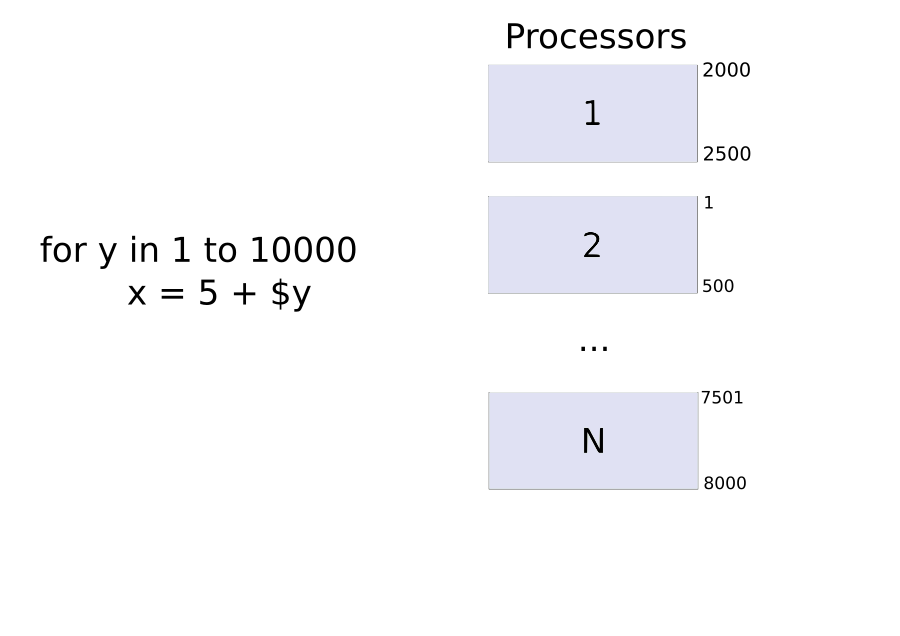
\includegraphics[width=0.8\linewidth]{figures/diagrams/forloop/fordiagram}
		\end{figure}	
\end{frame}

\begin{frame}
		\begin{figure}
				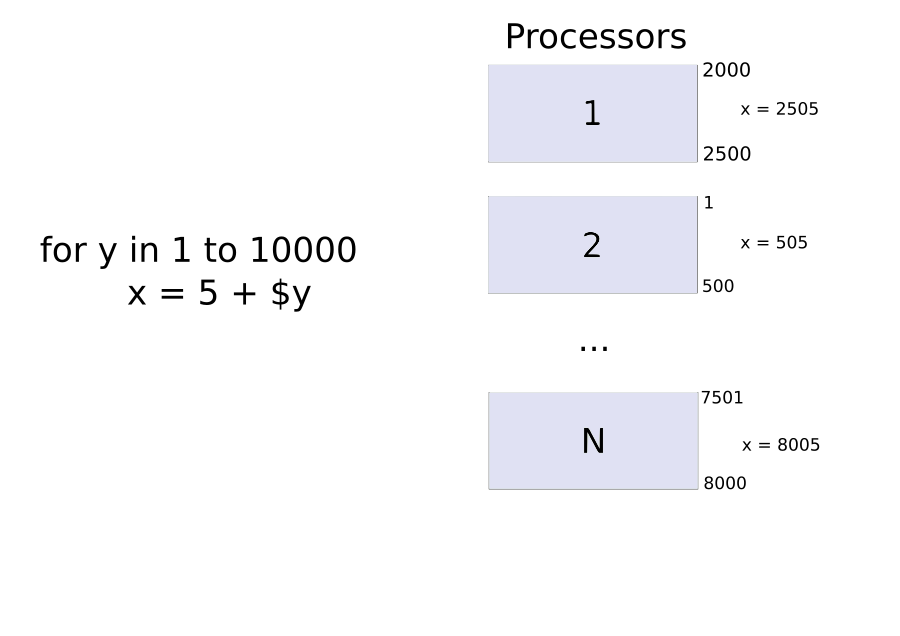
\includegraphics[width=0.8\linewidth]{figures/diagrams/forloop/fordiagram2}
		\end{figure}	
\end{frame}

\begin{frame}
		CLI examples of parallel utilities
\end{frame}

\begin{frame}
		parallel R for loop (code)
\end{frame}

\begin{frame}
		observed/expected speedup (figure)
\end{frame}

\begin{frame}
		Amdahl's law (code diagram)
\end{frame}

\begin{frame}
		Parallelization overhead (code diagram)
\end{frame}

